The usefulness of the Process Simulate application stems from its ability to verify the feasibility of an assembly process before breaking ground. Validating reachability and collision clearance is done by simulating the full assembly sequence of the product and the required instruments \cite{ProcessSimulateProductPage}. Figure~\ref{fig:ProcessSimulate} shows a screenshot of the application. \\

To walk the readers through Process Simulate, I put together this rather practical text.
It includes helpful tips and instructions should the reader want to follow along.
While the Process Simulate tool isn't widely available, SIEMENS offers a similar application, RobotExpert, with limited functionality, to which this text is applicable as well. \\

\subsection{Create a Study}
To begin working with Process Simulate one first has to set up his workspace. The content of every project is divided into two parts. A library and a study.
The library contains the models and specifics of the robots, tools, and others, while the study includes information about a specific space, a robotic cell perhaps, with instances of the models positioned within. \\

The first thing to create a project is to set up both your library and create a new study.
The library is set up at install time and will be shared for all of your studies.
Process Simulate will walk you through creating a new study. \\

I advise after creating a study to turn on floor rendering by selecting \emph{View \textgreater Screen Layout \textgreater Display Floor} in the ribbon menu. \\

\subsection{Inserting Components}
You can insert a component by selecting \emph{Modeling \textgreater Components \textgreater Insert Component} in the ribbon menu.
You will be prompted to select a folder containing your model. 
The supported folders have a name ending with \emph{.co} or \emph{.cojt} which signifies that they're in the proper format. \\

When inserting a component for the first time, you may receive an error saying that you needed to define its type. 
The fastest way to define a component's type is to enter the search commands and objects popup (Ctrl+F) and search for a \emph{Define Component Type} command.
You will be prompted to select a folder (the same folder as before) and then to choose the type of the component. Types offered include a robot, gun, container, etc.
The component will be inserted at the origin point in the study. \\

\subsection{Modeling}
Process Simulate offers a modest kit of modeling tools. 
Most of the tools are located in the \emph{Modeling} tab.
Before you can start creating geometries you need to select a modeling scope.
Modeling scope is a group to which the created geometries will belong.
You can select a modeling scope by selecting the component and pressing \emph{Modeling \textgreater Scope \textgreater Set Modeling Scope}.
You can have more than one component in a modeling scope, however, its recommended to end the modeling scope once you've finished altering it.
You can end a modeling scope similarly to starting it by pressing the \emph{Modeling \textgreater Scope \textgreater End Modeling} button. \\

Like any other CAD software, Process Simulate offers a suite of fundamental 3D modeling tools.
In the \emph{Components} group next to the familiar \emph{Insert Component} button, we can find commands for creating brand new components and resources. \\

In the next tab named \emph{Layout,} is mainly dedicated to tools for positioning the elements of the study.
Notably, the placement manipulator dialog can be accessed using a keyboard shortcut \emph{Alt+P}.
This group also contains the \emph{Create Frame} command for which there are several options how to specify a Frame.
Frames are oriented points that specify a separate coordinate system within the study, and they are crucial for defining, for example, where do robots hold their tools and so on. \\

Finally, the \emph{Geometry} group contains commands to create geometries and unify/subtract them together. \\

\subsection{Defining Kinematics}
Definition of kinematics is the process of defining parts of the model and linking them together with movable joints.
It is done using the \emph{Kinematics Editor}, which you can see in Figure~\ref{fig:KinematicsEditor}. This feature can be accessed using the \emph{Modeling \textgreater Kinematics \textgreater Kinematics Editor} command. \\

\begin{figure}[H]
    \caption{Kinematics Editor}
    \centering
    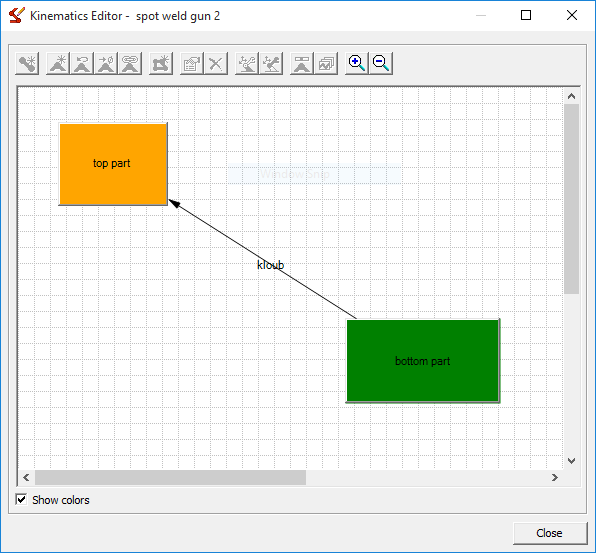
\includegraphics{kinematics_editor}
    \label{fig:KinematicsEditor}
\end{figure}

In the Kinematics Editor, the first button (\emph{Create Link}) will allow you to select all the geometries that belong to a single part.
Once there are multiple parts defined a joint can be established by dragging a mouse from a source part onto a destination part.
This order is significant in the definition of the joint. 
The source part will stay stationary while the destination part, to which the arrow is pointed, will be the one moving.
As a next step, it is necessary to define the axis of the movement and its limitations.
Once defined the joint can be tested in the \emph{Joint Jog} dialog. \\

\subsubsection{Poses}
A component or a resource can have several predefined poses. 
A pose is just an assignment of values for each joint which controls how rotated the joint is. 
Poses can be specified using the \emph{Pose Editor} dialog that has a button in the \emph{Kinematics} group. You can see the \emph{Pose Editor} in Figure~\ref{fig:PoseEditor}. Figure~\ref{fig:NewPose} shows how to define an new pose.\\

\begin{figure}[H]
    \caption{Pose Editor}
    \centering
    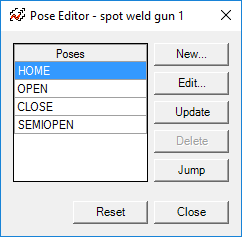
\includegraphics{pose_editor}
    \label{fig:PoseEditor}
\end{figure}
\begin{figure}[H]
    \caption{New Pose}
    \centering
    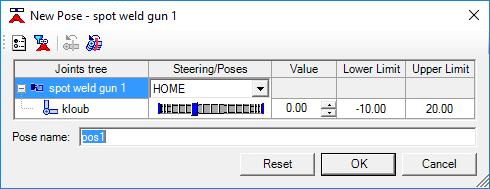
\includegraphics{new_pose}
    \label{fig:NewPose}
\end{figure}

\subsection{Robot Tools}
We can define a tool for a robot as a component.
Each tool type has a set of specific conventions that need to be followed for the application to know how to work with this tool. \\

Each gun type tool needs at least two frames. 
A mounting frame and an effector frame.
These can have arbitrary names. 
However, we will have to configure the robot to know which frame to use as an effector and which as a mounting frame.
The \emph{Mount frame} function specifies where and at what angle will the tool be connected to the robot.
Effector frame specifies where and what angle should the tool touch the product. \\

\subsubsection{Spot Welding Tool}
Each tool type has a few different quirks of its own.
The specific part about a spot welding gun is that it needs to have defined three poses to help the application generate a clamping animation.
These poses need to be named exactly \emph{HOME}, \emph{OPEN}, \emph{SEMIOPEN} and \emph{CLOSE}.
Even though it doesn't fit grammatically \emph{CLOSE} is correct without the N at the end, and doesn't work otherwise. \\

\subsubsection{Tool Definition}
Another step in creating tools is to define it as a tool.
We have already marked the component as a \emph{Gun}, \emph{Gripper} or another tool type, but we still need to assign a TCP. 
TCP stands for Tool Center Point, and it is a frame where the tool affects the product.
This dialog, shown in Figure~\ref{fig:ToolDefinition}, can be accessed using the \emph{Modeling \textgreater Kinematics \textgreater Tool Definition} command. \\

\begin{figure}[H]
    \caption{Tool Definition}
    \centering
    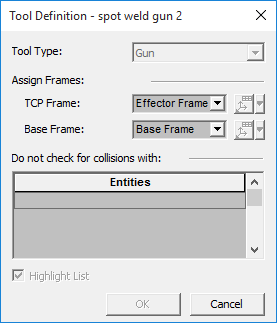
\includegraphics{tool_definition}
    \label{fig:ToolDefinition}
\end{figure}

\subsubsection{Mounting}
Now the tools are ready to be mounted.
We can do so using the mount dialog which can be accessed from the context menu (\emph{Right Mouse Button}) on the specific robot we want to mount the tool on and select \emph{Mount Tool}.
A dialog will be presented, as shown in Figure~\ref{fig:MountTool}.
Here, we need to specify what tool we need to mount, using which frame, on which robot and on which frame of the robot respectively.
Sometimes not all of the frames owned by the tool are displayed under the combo box. 
If this is the case enter modeling scope of the tool using the \emph{Set Modeling Scope} command and all the frames should now appear. \\

\begin{figure}[H]
    \caption{Mount Tool}
    \centering
    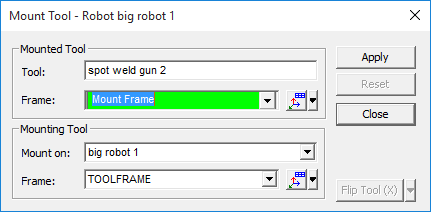
\includegraphics{mount_tool}
    \label{fig:MountTool}
\end{figure}

The second the two fields are related to the robot and should be prepopulated with the correct information.
If for some reason the robot wasn't well defined and doesn't contain a default tool frame you can set it here. \\

\subsubsection{Robot effector frame}
Last but not least we need to make sure the robot knows which frame to use to alter the product.
We can do this from the \emph{Robot Properties} dialog which can be accessed from the context menu of the robot by selecting the command with the same name. 
Here we set the TCP frame equal to the tools TCP frame.
In Figure~\ref{fig:RobotProperties} is a screenshot from this dialog of a correctly configured robot. \\

\begin{figure}[H]
    \caption{Robot Properties}
    \centering
    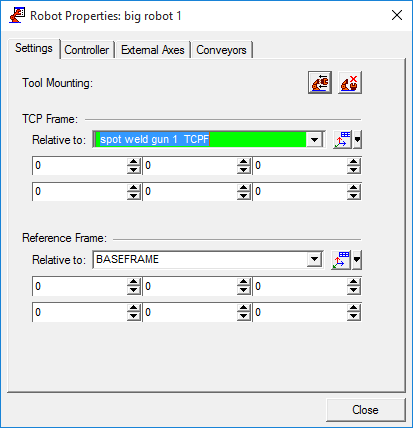
\includegraphics{robot_properties_toolframe}
    \label{fig:RobotProperties}
\end{figure}

\subsection{Positioning Robots}
There is nothing special on positioning robots as far as the basics go. 
Robots can be placed manually using the \emph{Placement manipulator} as any other components or resources.
For robots, however, Process Simulate includes several beneficial tools.
All of these tools are located as usual in the ribbon menu, in the \emph{Robot} tab.
I'd like to note a pair of them. \\

\subsubsection{Smart Place}
The Smart Place feature is located under \emph{Robot \textgreater Reach \textgreater Smart Place}.
It allows to quickly find places from which the specified robot will be able to reach all the specified points.
The feature works by making a grid around the robot and doing a reachability test for all the points in the grid.  
Aforementioned grid can be seen in Figure~\ref{fig:SmartPlace}.

\begin{figure}[H]
    \caption{Smart Place}
    \centering
    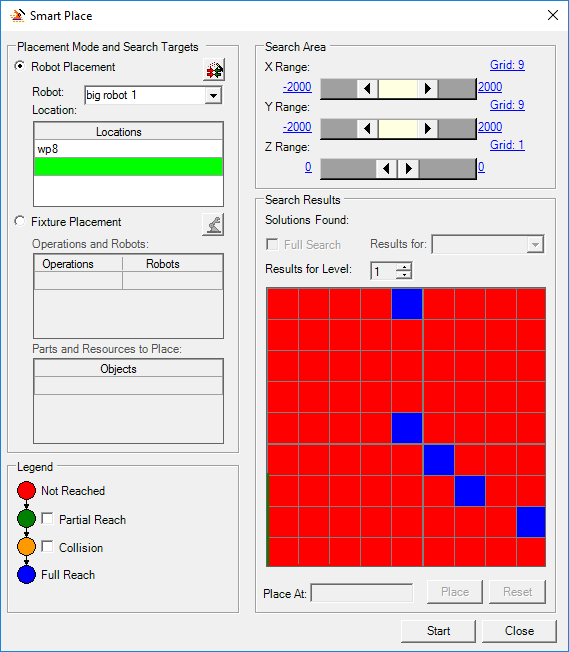
\includegraphics{smart_place}
    \label{fig:SmartPlace}
\end{figure}

\subsubsection{Reach test}
The Reach Test feature can be found under \emph{Robot \textgreater Reach \textgreater Reach Test}.
This feature allows testing given a robot and points out which operations he can or can't reach out of a specified list of operations.
Figure~\ref{fig:ReachTest} pictures the dialog controlling the feature.  \\

\begin{figure}[H]
    \caption{Reach Test}
    \centering
    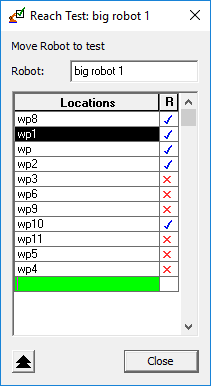
\includegraphics{reach_test}
    \label{fig:ReachTest}
\end{figure}

\subsection{Operations}
Operations are a way of defining movement for the robots.
The main view to interact with operations through is the \emph{Operations Tree} panel.
Operations have a root node and form a tree structure by nesting. The leaves of this tree we call points because they signify the individual locations in 3D space that the robot must visit. One layer above are operations which are linked to a robot and encompass a list of points. All the layers above are for logical grouping.
Although there are many types of operations, the best example of this is a \emph{Compound Operation} that makes up most layers above paths, including the root. \\

Commands for working with operations can be found on the \emph{Operations} tab. 
Some common operation commands are on the \emph{Home} tab. However, the \emph{Operations} tab contains those and more, which are necessary when creating welding operations. \\

\subsubsection{Compound Operation}
Compound Operation is a very simple but an essential building block.
It allows for grouping operations into a larger block and more importantly managing when and how long will each suboperation run.
It enables to run multiple child operations at the same time or having one operation start after another, even composing intricate timelines. \\

To start managing the timeline the operation needs to be set as a current operation. 
You can select an operation by highlighting it in the \emph{Operations Tree} and selecting \emph{Set Current Operation} from the mouse context menu or using the keyboard shortcut \emph{Shift + S}. \\

Process Simulate will then populate the \emph{Sequence Editor} panel (see Figure~\ref{fig:SequenceEditor}) with information about the newly set current operation. \\

\begin{figure}[H]
    \caption{Sequence Editor}
    \centering
    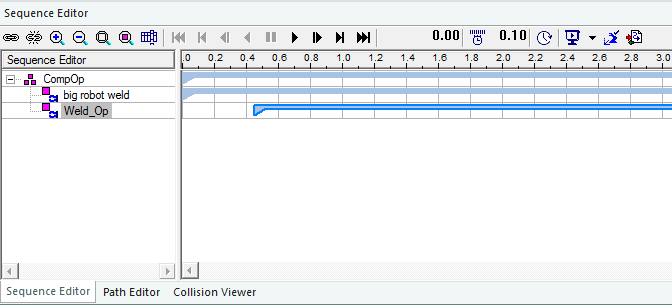
\includegraphics[width=\textwidth]{sequence_editor}
    \label{fig:SequenceEditor}
\end{figure}

The order of operations within a compound operation can be reordered by dragging and dropping inside the \emph{Operations Tree} panel.
This order is merely for convenience as it doesn't affect the order of execution.
For this, we have the \emph{Sequence Editor}. 
In this panel, each operation is represented by a blue bar next to the operations name in the left list. 
These bars are draggable and represent the start, the duration and the end of the operation. \\

\subsubsection{Device Operation}
Device operation moves a robot to a specific pose.
Which robot and into which pose should it move needs to be specified when it's being created.
This operation is mainly useful for returning robots into their home position so they can be ready for the next product after finishing work on the current one. \\

\subsubsection{Object Flow Operation}
Object Flow Operation moves an object from one place to another.
Process Simulate will present a dialog asking for a start frame, and an end frame (from and to) should the object be moved, similarly to other operations.
This operation is unique by not having to be assigned to a robot. \\

\subsubsection{Spot Weld Operation}
Spot welding in Process Simulate is separated into two parts: picking weld points, and combining weld points into weld operations.
Spots on the product that is to be spot welded need to be designated for welding.
This can be done using the \emph{Process \textgreater Discrete \textgreater Create Weld Point by Pick/Coordinates} command.
Clicking \emph{Create Weld Point by Coordinates} will present a dialog where one can fill coordinates and select on which part the weld will happen.
On the other hand \emph{Create Weld Point by Pick} will change a cursor and allow the user to pick points in the study where to weld. 
These points don't yet have a part associated with them so Process Simulate can compute a perpendicular angle from the part's surface and correctly guide the robot.
Unassociated points can be projected on a surface of a part using the \emph{Project Weld Points} command in the same command group. 
The user will be again presented with a dialog to select all the weld points to be projected and a list of parts to project them onto. \\

Once each point is created and projected on a part, an operation will appear for it.
This is where the second part comes in.
We need to create a weld operation (\emph{Operation \textgreater Create Operation \textgreater New Operation \textgreater New Weld Operation}), specify a robot to do the welding and populate its weld list.
That is a list of the individual weld point operations we just created in the first part.
The robot will then go in order of the atomic operations inside of the weld operation and process the points. \\

\subsection{Detecting Collisions}
Now that we defined our operations we can talk about simulating operations and detecting any problems that might occur when using that operation in the real world.
We are already familiar with the \emph{Sequence Editor} panel, of which will take further advantage. Furthermore, we'll explore the \emph{Collision Viewer} panel which is located in the same area.
Using the \emph{Collision Viewer} panel (see Figure~\ref{fig:CollisionViewer}) we need first to define what collisions to check.
Collision checking is a time-consuming process, so the fewer checks we have defined, the faster the simulation will go. \\

\begin{figure}[H]
    \caption{Collision Viewer}
    \centering
    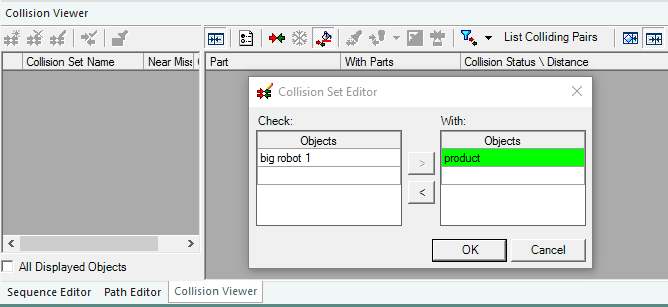
\includegraphics[width=\textwidth]{collision_viewer}
    \label{fig:CollisionViewer}
\end{figure}

To specify a new check, we use the \emph{New Collision Set} command which can be invoked by the first button in the \emph{Collision Viewer} panel.
You will be prompted to fill in for collisions of what objects with which objects (usually the robot and the product as depicted in Figure~\ref{fig:CollisionViewer}).
Note the \emph{Collision Options} command on the \emph{Collision Viewer}; the dialog contains options from tolerances to stop the simulation when a collision is detected.
Last but not least we need to make sure we have \emph{Collision Mode} enabled. 
This option is controlled by another button in the \emph{Collision Viewer} panel. \\

After we set up our collision detection, we can run the simulation.
We can do so from the \emph{Sequence Editor} by clicking the friendly looking play button. 
A simulation will now start moving the robots and when a collision happens a beep sound will be played unless configured otherwise. \\